% !TEX program = xelatex

\documentclass{resume}
\usepackage{graphicx}
\usepackage{tabu}
\usepackage{multirow}
\usepackage{progressbar}
%\usepackage{zh_CN-Adobefonts_external} % Simplified Chinese Support using external fonts (./fonts/zh_CN-Adobe/)
%\usepackage{zh_CN-Adobefonts_internal} % Simplified Chinese Support using system fonts

\begin{document}
\pagenumbering{gobble} % suppress displaying page number


{
% Adjust font size here
\Large{
  \begin{tabu}{l c }
    % Left side: Name and contact information
    \begin{tabu}{ l }
      \scshape{王小予} \\ % Name
      \email{xiao-yuwang@outlook.com} \textperiodcentered\ 
      \phone{(+86) 182-7377-0670} \textperiodcentered\ 
      \linkedin[XIAO-YU WANG]{https://www.linkedin.com/in/xiao-yu-wang-13a345330}
    \end{tabu}
    &
    % Right side: Photo
    \multirow{5}{1in}{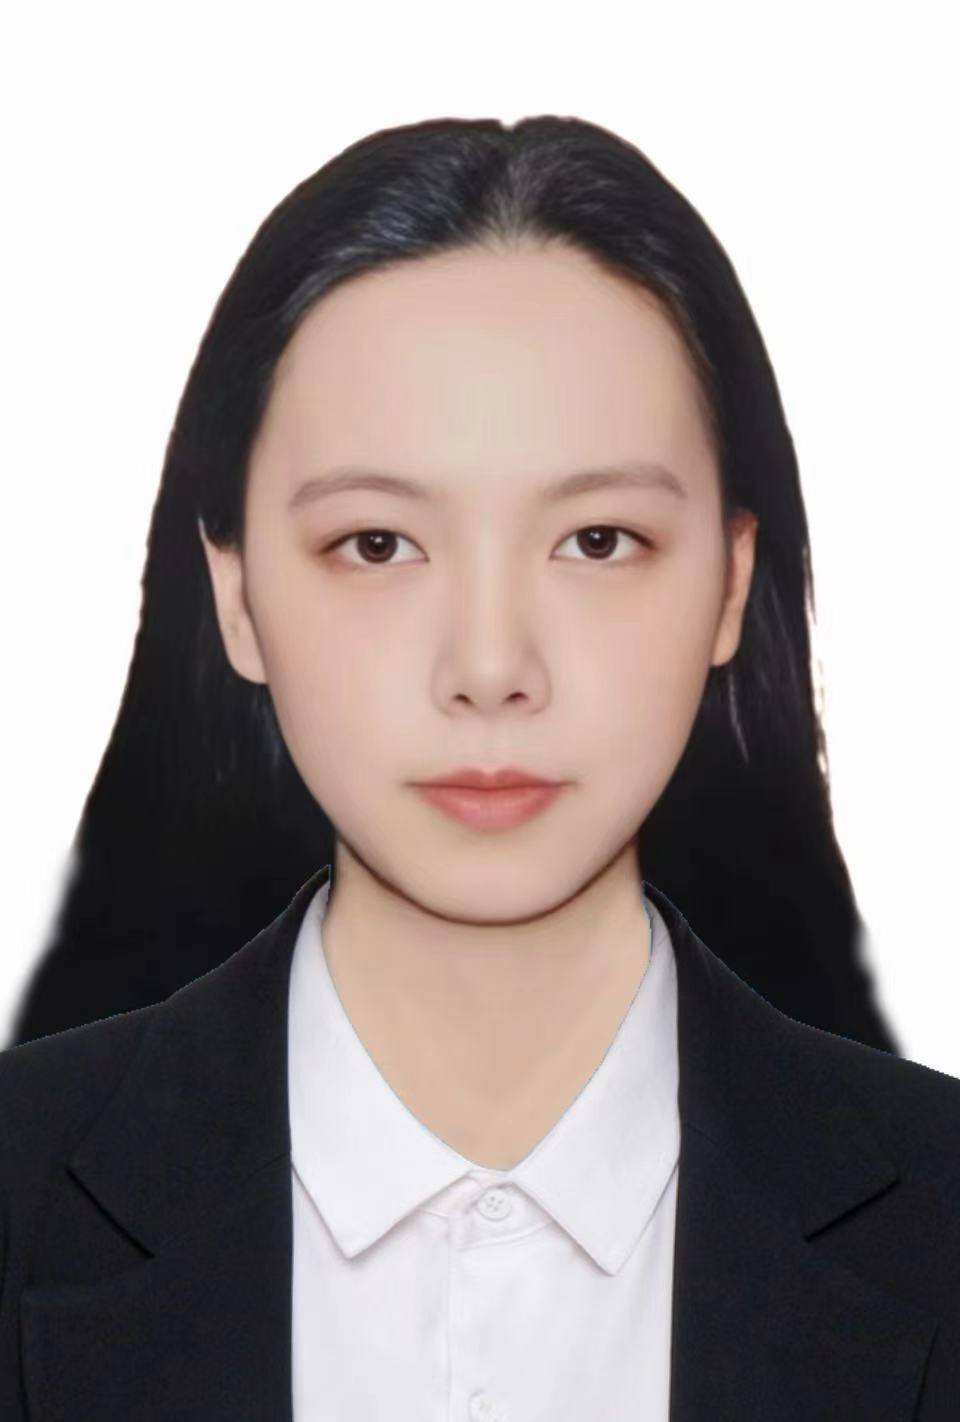
\includegraphics[width=0.88in]{photo}} % Replace 'avatar' with your photo file
  \end{tabu}
}
}


\section{\faGraduationCap\ Education}
\datedsubsection{\textbf{Tongji University (Tongji)}, Shanghai, China}{2022 -- Present}
\textit{B.S.} in Computer Science (CS), expected July 2026
\begin{itemize}
  \item GPA: 88.34/100
  \item Major Courses: Advanced Programming, Database Systems, Data Structures, AI (all 5.0/5.0)
\end{itemize}

\section{\faUsers\ Experience}
\datedsubsection{\textbf{Helmholtz Centre for Infection Research (HZI)} Germany (Remote)}{Dec. 2023 -- Present}
\role{Daily Intern}{Supervisor: Kun D. Huang}
Overview: Involved in microbial data analysis and bio-database construction.
\begin{itemize}
  \item Analyzed microbial data (400+ gut bacteria, 190+ patient samples) using Random Forest, achieving 76.93\% accuracy and contributed to a paper published in collaboration.  
  \item Currently developing a bio-database to organize 300+ patient samples and biochemical data, with a user-friendly front-end interface for efficient management by biologists.
\end{itemize}

\datedsubsection{\textbf{Elderly and Funeral Service Management Platform Database Design}}{May. 2024 -- Nov. 2024}
\role{Database Developer and Web Designer}{Individual Projects}
Overview: Designed and implemented a database system for elderly and funeral services.
\begin{itemize}
  \item Developed a relational database for 400+ elderly care institutions and 100+ funeral service providers, integrating emergency alerts and real-time health monitoring.  
  \item Integrated service ratings and feedback to optimize institutional management.
  \item Used MySQL, Python, Flask, HTML, CSS, JavaScript for full-stack implementation.
\end{itemize}

\datedsubsection{\textbf{Data Modeling Competition(APMCM)}}{Oct. 2023 -- Jan. 2024}
\role{Team Leader}{Competition Project}
Overview: Led a team in a computer vision task for apple variety classification. 
\begin{itemize}
  \item Led a team of 3 to develop a fruit image recognition system for apple detection, ripeness estimation, and differentiation, trained on 10,000+ images with 90\% accuracy using YOLO and RESNET models.  
  \item Enhanced team communication, completing the project 12 hours ahead of the 3-day deadline.
\end{itemize}

% Reference Test
%\datedsubsection{\textbf{Paper Title\cite{zaharia2012resilient}}}{May. 2015}
%An xxx optimized for xxx\cite{verma2015large}
%\begin{itemize}
%  \item main contribution
%\end{itemize}

\section{\faCogs\ Skills}
\begin{itemize}[parsep=0.5ex]
  \item Programming Languages: C, C++, Python
  \item Platforms: Windows, Linux
  \item Development: Frontend (HTML/CSS, JavaScript); Backend (Node.js, Flask); Database (MySQL)
  \item Tools \& Frameworks: Git, Docker, PyTorch
  \item Computer Science Fundamentals: Operating Systems, Databases, Algorithms, Computer Networks
\end{itemize}

\section{\faHeartO\ Honors and Awards}
\datedline{\textit{\nth{3} Prize}, Award on Outstanding Undergraduate Student Scholarship, Tongji University}{Dec. 2023}
\datedline{\textit{\nth{3} Prize}, Award on APMCM (Asia-Pacific Mathematical Contest in Modeling) }{Jan. 2024}

\section{\faInfo\ Miscellaneous}
\begin{itemize}[parsep=0.5ex]
  \item GitHub: https://github.com/hoshigawarei
  \item Languages: English - Fluent (TOEFL:98), Mandarin - Native speaker
\end{itemize}

%% Reference
%\newpage
%\bibliographystyle{IEEETran}
%\bibliography{mycite}
\end{document}
